%%%%%%%%%%%%%%%%%%%%%%%%%%%%%%%%%%%%%%%%%%%%%%%%%%%%%%%%%%%%%%%%%%%%%%%%%%%%%%%%
%2345678901234567890123456789012345678901234567890123456789012345678901234567890
%        1         2         3         4         5         6         7         8
% THESIS INTRODUCTION

\chapter{Introduction}
\label{chap:introduction}
\ifpdf
    \graphicspath{{Introduction/Figures/PNG/}{Introduction/Figures/PDF/}{Introduction/Figures/}}
\else
    \graphicspath{{Introduction/Figures/EPS/}{Introduction/Figures/}}
\fi

% quote

%\setlength{\epigraphwidth}{.35\textwidth}
%\epigraph{Research is formalized curiosity.}{ Zora Neale Hurston, 1942}

% examples of sections

\section{Motivations}
\label{motivations}
A dynamic network changes over time. This could be changes in the network topology - that is, the existence of edges and existence of nodes \cite{itdn}, or it could be changes in attributes associated with edges and nodes. Dynamic networks can be found everywhere: a road network which undergoes periodic maintenance to sections or junctions; a brain network where neuron activity varies; or a social proximity network where edges are created while people are close to each other and lost when they move apart.

Naturally, dynamic networks are difficult to quickly interpret and visualise \cite{iddps}. Consider even a simple network composed of a handful of nodes and a handful of edges. Suppose we add the dynamic element to this simple network and mutate, say, the edges through a given time period. It can be difficult to interpret what if anything those mutations indicate or represent even on a simple network. Many different approaches have been made to try and tackle this problem and mitigate the additional cognitive load. This report will focus on a novel approach - using a variety of easily interpretable measures to produce some result based on either an aspect of the graph at each frame of time or on the graph overall, for example: the density of the graph. Instead of manually stepping through the graph and attempting to pattern match, the measures can be observed instead. Similar to feature projection, this serves to effectively reduce the dimensionality \cite{wikidimred} of the problem down to the number of measures used as they provide an abstract overview of the changes the graph goes through. However as more and more measures are used we find ourselves with a similar complexity problem, and to remedy this an intelligent visualisation of the measure results must be implemented. Visualising these measures can allow us to spot patterns and trends over time, locate points of interest and motivate a hypothesis. Traditionally, network visualisations have been focused on visualising the changes themselves \cite{tsotaivg}, however here the measure-based approach aims to be more complementary to the network.

Although any type of network could have been used - care was taken while designing the measures and visualisations to keep them agnostic of the domain and avoid overfitting - a fairly small and simple social network was primarily used during development. 
%Social networks require less expert domain knowledge compared with say, biological networks to understand at a basic level [source or remove]. For the sake of simplicity I chose an easy to understand and rather small network. 
%Social networks are also more abstract than physical networks like power grids or computer networks \cite{taasodnv}.
Since this project aims to investigate dynamic network interpretation, using a simple network as a baseline ensures that difficulties in comprehension aren’t just inherent to the domain but to the network itself. 
%There are also a variety of existing networks that could be used to test against [source/example].
%Social network analysis provides a novel window by allowing the impacts to be quantified at the individual level, and the links between past, current and future behaviour to be carried across contexts. <https://besjournals.onlinelibrary.wiley.com/doi/pdf/10.1111/1365-2656.12764>

I extend the functionality of The Vistorian \cite{bach:hal-01205822} - an ongoing open source project by Benjamin Bach, Nathalie Henry Riche, Roland Fernandez, Emmanoulis Giannisakis, Bongshin Lee, et al to create an online platform which provides interactive visualization for various kinds of networks, designed for social scientists and historians. 

Networks can be constructed and interpreted in different ways. The measures used in this report are designed for a network composed of eternal nodes, unweighted and undirected edges, where an edge is a connection that happens instantaneously between two nodes, as in type (a) of Figure \ref{fig:edgeTypes}, and a nodepair exists between two nodes in a given period of time if any edge occurs between them in that period. 

\begin{center}
\begin{tabular}{cc}
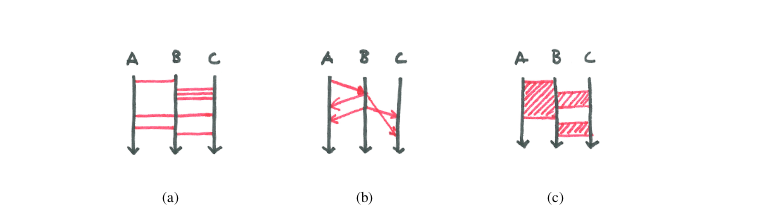
\includegraphics[trim={0 0 0 0}, width=140mm]{./Figures/edgeTypes.png}
\end{tabular}
\captionof{figure}{Types of connectivity. A, B and C represent nodes, time goes from top to
bottom, edges are indicated in red. (a) Instantaneous edges, (b) Transmissive edges, (c)
Persistent edges. \newline Figure and description taken from Connections, Changes and Cubes: Unfolding Dynamic Networks for Visual Exploration \cite{cccudnfve}.
}
\label{fig:edgeTypes}
\end{center}


Adjusting any of these assumptions would affect the selection of measures. Further work could be done on measures that take into account edge weight, persistent edges etc. The measures are also designed with social networks in mind, but could of course be applied in other domains.



\section{Objectives and Contributions}
\label{objectives}
\begin{itemize}
    \item Summary of the literature regarding dynamic network visualisation.
    \item Development and evaluation of novel local dynamic measures - Local volatility, local activity and local redundancy.
    \item Development and evaluation of novel global dynamic measures - Global volatility, global activity and global redundancy.
    \item Extension of The Vistorian through:
    \begin{itemize}
        \item Implementation of methods to calculate measures.
        \item Creating a visualisation of these measures, embedded into the existing interface.
        \item Implementing an extensible framework that ensures new global measures can be easily visualised.
    \end{itemize}
    \item Demonstration of visualisations and measures in usage scenarios.


\end{itemize}





